\documentclass[conference]{IEEEtran}
\IEEEoverridecommandlockouts
\usepackage{amsmath,amssymb,booktabs,multirow,graphicx}
\usepackage{array}
\usepackage{url}
\usepackage{xcolor}
\usepackage[hidelinks]{hyperref}
\usepackage{balance}
\graphicspath{{figures/}}
\newcommand{\Aclass}{A}
\newcommand{\Bclass}{B}
\newcommand{\Cclass}{C}
\newcommand{\RF}{random forest}
\newcommand{\OOF}{out-of-fold}
\newcommand{\CtoA}{C$\rightarrow$A}

\title{Safety-Aware Multi-Objective Transparent Evaluation of Levee Seepage Stability: Integrating Geological, Seepage-Field, and UAV Inspection Evidence}

\author{\IEEEauthorblockN{Author names and affiliations to be completed}
\IEEEauthorblockA{Internal working manuscript, September 2026\\
Corresponding author: to be completed}}

\begin{document}
\maketitle

\begin{abstract}
Levee seepage evaluation is often compressed into a final grade, while the geological evidence, simulated seepage field, inspection observations, and decision rules that produced the grade remain difficult to audit. We formulate transparent evaluation as a traceable decision chain from evidence state and provenance to indicator transformation, failure-mode response, risk grade, and triggering rule. The framework separates three roles that are frequently conflated in digital-twin workflows: the physics-based rule chain defines admissible safety constraints, a random-forest layer estimates nonlinear interactions among heterogeneous indicators, and a Pareto decision layer exposes the trade-off among classification quality, critical-class recall, dangerous underestimation, and review burden. The method was evaluated on 875 controlled synthetic scenarios spanning seven target modes and five severity levels, five additional generator realizations from the same controlled family, and a field infrared inspection set used to test the status handling of candidate piping detections. The reproduced rule baseline achieved 0.8446 accuracy, 0.8272 macro-F1, and 0.8371 recall for the critical class C. A grouped five-fold out-of-fold random forest increased class-C recall to 0.8543 but did not replace the rule baseline in aggregate performance. A representative threshold policy reached 0.8731 accuracy and 0.8584 macro-F1 in the original controlled batch, but introduced 50 direct C-to-A underestimates. A physical-veto hybrid that imposed the rule-model grade as a lower risk bound reached 0.9257 accuracy, 0.9119 macro-F1, and 1.0000 class-C recall with zero C-class underestimates in that batch; across five additional realizations, it achieved 0.9214$\pm$0.0042 accuracy and 0.9983$\pm$0.0038 class-C recall. A lower-review operating point routed 1.53$\pm$0.67\% of records to review while retaining 0.9903$\pm$0.0080 C recall in the same controlled family. Nine field detections were rejected during manual review, showing why algorithmic candidates cannot be injected into an evaluation as confirmed piping. The results establish a reproducible decision protocol and quantify its safety--performance trade-offs; they do not constitute independent field generalization evidence.
\end{abstract}

\begin{IEEEkeywords}
levee seepage, transparent evaluation, digital twin, random forest, Pareto optimization, piping detection, evidence traceability
\end{IEEEkeywords}

\section{Introduction}
Levee seepage safety is governed by the interaction of heterogeneous soil layers, hydraulic boundary conditions, transient water levels, local gradients, slope stability, and visible or thermal signs of abnormal discharge. A single safety grade is useful for operation, but it is insufficient for diagnosing why a grade was produced or whether the underlying evidence is current, applicable, and spatially aligned. This limitation becomes more consequential when a levee digital twin combines three-dimensional geology, numerical seepage computation, and airborne inspection: a visually convincing scene can still conceal an ambiguous indicator, a stale observation, or a rule that is not valid for the evaluated location.

Existing levee and dam assessment methods provide strong components for individual tasks. Numerical seepage models resolve hydraulic gradients and pore-pressure responses; reliability methods propagate parameter variability; and computer-vision systems detect candidate leakage or piping signatures. However, these components are commonly evaluated with different data models and different notions of truth. The final grade therefore becomes difficult to reproduce when a geological property, a computed field value, and an inspection box are merged without an explicit evidence state. In addition, a data-driven classifier can improve aggregate accuracy while increasing the probability of a safety-critical downgrade from class C to class A. Digital-twin research emphasizes synchronization between a physical asset and its virtual representation, but synchronization alone does not define whether a stale, unregistered, or merely suspected observation is admissible for a safety decision~\cite{Fuller2020}.

We address this gap by treating transparent evaluation as an auditable decision problem rather than as a display function. The evaluation unit is defined by a section, hydraulic scenario, time, and evidence version. Every indicator retains its raw value, unit, source, applicability, availability, spatial and temporal scope, and transformation rule. Physics-based gates remain authoritative for known critical conditions. A machine-learning layer is used as a controlled comparator and as a probability estimator, not as an unrestricted replacement for the physical model. A Pareto policy then exposes the trade-off among aggregate classification quality, critical-class recall, dangerous underestimation, and escalation burden. This formulation leads to three testable questions: whether a nonlinear comparator improves the closed-set classification metrics; whether it changes the direction of errors in safety-critical cases; and whether an explicit physical lower bound or reject state can preserve safety while limiting unnecessary escalation.

The paper makes five contributions. First, it formalizes an evidence-state and provenance model for integrating geological, seepage-field, and UAV inspection information. Second, it defines a reproducible benchmark in which duplicate physical feature vectors are grouped during cross-validation and target labels are derived from the frozen scenario severity rather than from delivered model outputs. Third, it compares a shallow decision tree and a random forest with the reproduced rule baseline and evaluates threshold policies through Pareto dominance and a safety loss. Fourth, it introduces a physics-veto hybrid that prevents the learned policy from lowering an existing physical risk grade. Fifth, it reports the current boundary of field evidence: nine reviewed field detections were false positives, while the remaining images and validation images do not yet provide a complete image-level truth set.

\section{Related Work and Research Gap}
\subsection{Geological and numerical representations}
Implicit geological modeling provides a compact way to interpolate stratigraphic interfaces from boreholes, sections, and structural observations. Reviews of three-dimensional structural models emphasize that the interpolation method, conditioning data, and geological uncertainty are inseparable from the resulting geometry~\cite{Wellmann2018}. Open-source implementations such as GemPy make geological interpolation and visualization accessible and support arbitrary slicing of a three-dimensional model~\cite{GemPy}. For seepage analysis, however, the geological representation must be converted into material zones, hydraulic properties, and a mesh or solver grid. The conversion is a potential source of silent inconsistency: a layer that is visible in the geological scene may not be represented in the numerical domain, and a numerical maximum may be extracted from a region whose material identity is unknown. A transparent workflow must therefore preserve the mapping from geological surface to numerical material, rather than treating the rendered model as evidence of numerical consistency.

\subsection{Digital twins and provenance-aware infrastructure models}
Digital-twin studies commonly describe a loop linking sensing, model updating, simulation, and decision support~\cite{Fuller2020}. For levees, the difficult part is not only maintaining a three-dimensional scene but also maintaining the identity, validity interval, and spatial support of every observation that enters the scene. BIM- and mechanism-based levee studies similarly motivate lifecycle integration, yet they do not by themselves solve the admissibility problem for incomplete or conflicting evidence~\cite{Hou}. We therefore use the digital twin as an information and visualization context, while defining the safety decision through explicit evidence states and versioned transformations.

\subsection{Seepage safety and uncertainty}
Transient seepage is commonly described by Richards-type formulations~\cite{Richards,Celia1990}, with unsaturated hydraulic properties often represented through constitutive relationships such as the van Genuchten model~\cite{vanGenuchten1980} or related soil--water characteristic curves. Saturated-flow reductions are useful for operational screening, but the choice of formulation, hydraulic parameters, boundary conditions, and extraction region can change the interpretation of a local gradient. Reliability and Bayesian approaches can incorporate spatial variability and field observations~\cite{Xu,Schweckendiek,Roscoe,Baecher2003}, but they do not by themselves specify how an inspection candidate, a missing observation, or an inapplicable indicator should alter the final operational grade. A transparent evaluation layer must therefore preserve both the numerical response and its evidence status, including the distinction between model uncertainty, observation uncertainty, and evidence absence.

\subsection{Inspection and data-driven decision support}
UAV and infrared inspection can cover long levee reaches and provide candidate locations for follow-up; the broader remote-sensing literature also shows that georegistration, radiometric calibration, and flight metadata determine whether an image can support a spatial engineering inference~\cite{Colomina2014}. Image segmentation and object detection methods such as U-Net~\cite{Ronneberger2015} and YOLO~\cite{Redmon2016} are effective for screening, but thermal contrast from water boundaries, vegetation, shadow, wet soil, buildings, and lens effects can mimic a piping signature. Manual review and spatial registration are therefore part of the safety decision, not post-processing details. Tree-based models such as decision trees and random forests~\cite{Quinlan,Breiman,Hastie2009} are attractive for a complementary decision layer because they can represent nonlinear interactions and provide probability estimates and feature-level inspection~\cite{LundbergLee}, yet their use in safety assessment requires explicit control of false-safe decisions. Because the classes are ordinal and the cost of a critical downgrade is asymmetric, macro-F1, balanced accuracy, and precision--recall behavior are more informative than accuracy alone~\cite{Saito2015}.

\subsection{Evidence fusion and the remaining gap}
Evidence-fusion formalisms, including Dempster--Shafer theory, provide a language for combining partially specified support and ignorance~\cite{Shafer1976}. Their use in engineering evaluation does not remove the need to define when evidence is applicable, how conflicts are handled, or whether a candidate observation is sufficiently localized to constrain a current state. The unresolved issue is therefore not the absence of a classifier or a visualization platform. It is the lack of a common, traceable decision protocol that (i) distinguishes unavailable, inapplicable, suspected, and confirmed evidence; (ii) compares data-driven predictions with a physics-based rule chain under leakage-safe validation; and (iii) makes the cost of a critical-class downgrade explicit.

\subsection{Gap addressed in this study}
We use the 875-scenario controlled package as a reproducibility benchmark and use the field inspection records to test the evidence-state interface, while keeping engineering generalization claims separate from controlled behavior. The study is consequently positioned as a decision-layer and protocol contribution: it asks how heterogeneous evidence should be represented and constrained before it is visualized or fused, rather than claiming that a classifier trained on a controlled package has already generalized to unseen levees.

\section{Transparent Evaluation Framework}
\subsection{Evaluation unit and evidence states}
An evaluation record is indexed by the tuple $(s,w,t,v)$, where $s$ denotes the levee section, $w$ the hydraulic scenario, $t$ the observation or simulation time, and $v$ the evidence and rule version. The record contains the indicator code, raw value, unit, transformed score, source location, value type, applicability, availability, time window, spatial support, and transformation rule. The value type distinguishes direct measurements, numerical outputs, representative assignments, controlled synthetic values, and manual assignments.

Applicability and availability are kept as separate fields. An indicator is marked \emph{inapplicable} only after the relevant facility or failure mode has been confirmed absent; it is marked \emph{missing} when the indicator should be evaluated but evidence was not obtained. Neither state is silently encoded as a zero or a perfect score. For inspection evidence, three states are retained: algorithmic candidate, manually reviewed status, and evaluation input. Only an event with closed temporal and spatial correspondence can impose a deterministic defect or piping constraint on the current evaluation unit.

Table~\ref{tab:evidence} summarizes the main evidence channels used in this study.

\begin{table}[t]
\caption{Evidence channels and their admissibility in transparent evaluation.}
\label{tab:evidence}
\centering
\scriptsize
\setlength{\tabcolsep}{2pt}\begin{tabular}{@{}p{0.18\columnwidth}p{0.25\columnwidth}p{0.39\columnwidth}@{}}
\toprule
Channel & Example evidence & Admissibility condition \\
\midrule
Geology & control layer, soil properties, contact zone & spatially registered and material identity retained \\
Seepage field & local gradient, critical-gradient ratio, FoS & boundary condition, scenario, extraction region, and material known \\
Inspection & candidate box, confidence, review status & time, location, and review state explicitly stored \\
History & previous piping or seepage event & event time and current relevance distinguished \\
Missingness & unavailable or stale input & reported as an evidence state with a missing-item list \\
\bottomrule
\end{tabular}
\end{table}

\subsection{Provenance graph and alignment operator}
The evidence table is implemented as a directed provenance graph rather than as a flat list of values. A node represents an observation, a geological object, a numerical field, a review action, or a decision output; an edge records derivation, spatial registration, temporal precedence, or rule triggering. For an evaluation unit $(s,w,t,v)$, an indicator $x_j$ is admissible only when its support intersects the unit, its validity interval contains $t$, and its version $v_j$ is compatible with the evaluation version. We represent this condition with
\begin{equation}
 a_j(s,w,t,v)=\mathbf{1}\{\mathcal{S}_j\cap\mathcal{S}_s\neq\varnothing\}\,\mathbf{1}\{t\in\mathcal{T}_j\}\,\mathbf{1}\{v_j\preceq v\},
 \label{eq:admissibility}
\end{equation}
where $\mathcal{S}_j$ and $\mathcal{T}_j$ are the spatial support and validity interval of the indicator. If $a_j=0$, the value is retained for traceability but cannot silently become a normal score. This representation makes a spatially misregistered inspection box and a stale simulation output visible as provenance failures rather than as numerical zeros.

The same rule is applied to model outputs. A local seepage maximum is linked to the material zone and extraction region from which it was computed; an inspection candidate is linked to its image, timestamp, camera position, and review record; and a historical event is linked to the event interval rather than copied into every later evaluation. This design follows the broader digital-twin requirement that state synchronization must preserve identity and context, but it adds an explicit admissibility gate for safety evaluation~\cite{Fuller2020}.

\subsection{Physics-based score and grade}
The existing evaluation model contains 29 secondary indicators and five failure modes: overtopping, seepage, slope instability, scour, and through-structure effects. Let $R_m\in[0,1]$ be the management-barrier-adjusted response for failure mode $m$, $\pi_m$ its normalized weight, and $\alpha$ the shortfall coefficient. The composite risk measure and score are
\begin{equation}
\rho=\alpha\max_m R_m+(1-\alpha)\sum_m \pi_m R_m,
\label{eq:risk}
\end{equation}
\begin{equation}
S=100(1-\rho).
\label{eq:score}
\end{equation}
The reproduced baseline uses $\alpha=0.45$. The raw grade is A for $S\geq80$, B for $40\leq S<80$, and C for $S<40$. An observation upper bound and physical hard gates are then applied in sequence. The gates cover overtopping, the C1/C4/C5 seepage indicators, slope factors of safety, scour, structures, and settlement. The final grade is allowed to remain unchanged or move toward a higher-risk class; it cannot be made safer by a conflicting observation rule.

The seepage indicators C1, C4, and C5 are associated with the foundation, embankment, and contact zone, respectively. A local maximum is admissible only when its extraction region and material identity are retained. The dominant failure mode is reported as the largest internal response and is not interpreted as a calibrated failure probability.

\subsection{Machine-learning comparator}
We trained a shallow decision tree and a random forest using 14 features derived from the physical and inspection channels: crest elevation, foundation/body/contact gradients, upstream and downstream factors of safety, scour depth, inspection density and level, and their normalized ratios or inverse factors of safety. The feature exclusion list contains target mode, target severity, grade, model grade, composite score, risk measure, dominant mode, and all delivered model outputs. The target class is derived from the frozen scenario severity: safe and slight map to A, moderate maps to B, and severe and critical map to C. The reference forest used 120 trees, maximum depth 7, minimum leaf size 3, and four randomly selected features per split. These settings were fixed before the five additional generator realizations and were not retuned for the reported seed means.

Because the controlled package contains repeated physical feature vectors, all identical vectors are assigned to the same cross-validation fold. We use grouped five-fold out-of-fold (OOF) predictions. The random forest probability vector $p=(p_A,p_B,p_C)$ is retained for threshold selection; majority voting is used as the untuned machine-learning comparator.

The probability vector is used as a decision-support object rather than as a calibrated failure probability. A high $p_C$ indicates that the learned model favors the critical class under the controlled target construction; it does not imply that the field probability of piping is $p_C$. This distinction is important because the benchmark labels are generated from scenario severity, whereas a field label would require an independently timed and spatially registered observation.

\subsection{Metrics, error direction, and paired comparison}
For each class $k$, precision and recall are computed from the held-out predictions, and macro-F1 is the unweighted mean of the three class-specific F1 scores. Balanced accuracy is the mean recall over A, B, and C. We additionally report the number of C-class underestimates, the direct C-to-A count, the A-class overestimate count, and the review rate. These metrics separate ordinary classification quality from the direction and operational burden of errors. Because only five additional generator realizations were available, multi-seed results are summarized as paired means and standard deviations; no inferential claim is made from a small number of synthetic seeds.

\subsection{Pareto decision layer}
For a candidate pair $(\tau_C,\tau_B)$, the policy is
\begin{equation}
\hat y=\begin{cases}
C,&p_C\geq\tau_C,\\
B,&p_C<\tau_C\ \text{and}\ p_B\geq\tau_B,\\
A,&\text{otherwise.}
\end{cases}
\label{eq:threshold}
\end{equation}
Candidate policies are compared using accuracy, macro-F1, balanced accuracy, recall for C, C-class underestimates, direct C-to-A underestimates, A-class overestimates, and escalation rate. To expose the operational asymmetry, we define
\begin{equation}
L_{\mathrm{safe}}=2N(C\rightarrow A)+N(C\rightarrow B),
\label{eq:safeloss}
\end{equation}
where a direct C-to-A decision is assigned twice the loss of a one-level C-to-B downgrade. The Pareto set contains non-dominated policies over aggregate quality, critical recall, safety loss, and escalation, following the standard logic of multi-objective optimization~\cite{Deb}. Physical hard gates and evidence completeness checks have priority over the learned policy.

For the representative RF operating point reported below, we first required zero A-class overestimates and C recall of at least 0.85 on the exploratory $0.05$ threshold grid, and then selected the point with the largest macro-F1. This yields $(\tau_C,\tau_B)=(0.35,0.20)$. It is a declared operating point rather than an independently optimized engineering policy. A finer $0.01$-grid audit is used to test whether the learned threshold layer alone can satisfy the stronger direct C-to-A constraint.

\subsection{Physics-veto hybrid policy}
The grade labels are ordinal for decision purposes, with A, B, and C encoded as 0, 1, and 2. Let $\hat y_{\mathrm{RF}}$ be a learned prediction from Eq.~(\ref{eq:threshold}) and let $y_{\mathrm{rule}}$ be the final grade returned by the existing physics-based rule chain. We define a monotone physical-veto hybrid as
\begin{equation}
\hat y_{\mathrm{hyb}}=\max\left(\hat y_{\mathrm{RF}}, y_{\mathrm{rule}}\right).
\label{eq:veto}
\end{equation}
The operation is a decision-layer lower bound: the learned model may escalate a rule result, but it cannot make the result safer. It does not retrain either component and it leaves the evidence trace and triggered physical gate intact. The construction is monotone with respect to the ordinal risk order, but it does not claim that the rule output is a calibrated probability or an error-free truth label. As an operational variant, predictions with $\max_c p_c<u$ are routed to review and use $y_{\mathrm{rule}}$ as a fallback. The review rate and the fallback metrics are reported separately from the hybrid's closed-set classification metrics. In the exploratory budget analysis, $u=0.50$ and $u=0.60$ are compared to expose the cost of demanding a more confident learned output.

\section{Data and Validation Protocol}
\subsection{Controlled 875-scenario benchmark}
The benchmark was generated with a frozen random seed and contains 875 records: seven target modes, five severity levels, and 25 records per mode--severity combination. The reference class is defined by the scenario severity and is used only to test behavior under the controlled generator. It is not a field safety label. The authoritative rule baseline is reconstructed from the final-grade error trace, rather than from the raw grade column in the input CSV.

We report accuracy, macro-F1, balanced accuracy, per-class precision and recall, C underestimates, A overestimates, and the confusion matrix. We also preserve the original score grade, observation upper-bound grade, final grade, and triggered gate for each record. All machine-learning results in the main text are controlled-batch results; a five-outer by three-inner grouped nested validation prototype is reported as a robustness check. The physical-veto hybrid uses the fixed delivered rule output only at the decision layer and uses the OOF learned prediction for each held-out fold.

The validation hierarchy is deliberately separated into three levels. The original 875 records test reconstruction against the frozen reference; the five additional batches test sensitivity to the generator realization; and the inspection and engineering packages test whether evidence states and provenance fields can be carried through the interface. None of the latter packages is used to claim external predictive accuracy. In particular, a reviewed field candidate is evidence about that candidate's status, not a complete denominator for image-level detection performance.

\subsection{Implementation and reproducibility controls}
The analysis scripts use deterministic random seeds and write the feature manifest, fold assignments, threshold grid, per-record predictions, and summary metrics. The five additional batches use seeds 20260930--20260934; the forest seed is derived from the fold index and held fixed across methods. The fine safety audit enumerates 10,000 pure-RF threshold pairs on a 0.01 grid, while the multi-objective exploratory grid uses 0.05 increments. These grids are reported to make the search space auditable, not to imply that the selected point is an engineering optimum. The source package also preserves the original rule output, the physical-veto output, and the review-fallback output for each record, allowing every aggregate metric to be reconstructed from a confusion matrix.

\subsection{Scope of the reference labels}
The target class is a closed-set reference derived from controlled scenario severity. It is useful for testing whether a decision layer responds in the intended direction, but it is not equivalent to a field diagnosis. This distinction is especially important for the critical class: a zero C-to-A count in the controlled benchmark verifies the behavior of the imposed decision constraint under the available reference labels; it does not prove zero false-safe decisions in an unseen levee. We therefore report the physical-veto result as a safety-constrained architecture result and state the missing external validation as a boundary of the present study.

\subsection{UAV and infrared inspection records}
The inspection package contains 114 field infrared images and associated visualizations, nine reviewed field detections, 13 artificial validation images, and 14 validation detections. The nine field candidates were all classified as false positives during manual review. The reported causes include water-boundary contrast, vegetation and shadow, building thermal inertia, wet ground, and lens-edge effects. The remaining field images do not yet have image-level truth labels, and the validation images do not provide a complete positive-boundary and missed-detection record. We therefore report the review-subset result as 0/9 confirmed piping and do not report field-wide accuracy, recall, or F1.

\subsection{Engineering case trace}
The K45+500 delivery case is used to test provenance and interface fields. It reports a representative high-water level of 35.90~m, a deep silty-clay controlling ratio of approximately 1.045, a downstream slope factor of safety of approximately 1.155, a composite score of 24.3481, and a C-grade seepage-dominant result. These values are delivery-result excerpts rather than an independent physical re-run. The case also contains unresolved conflicts between the 29-indicator table and the result JSON and includes historical piping information in the input. It is therefore not treated as a blind test.

\section{Results}
\subsection{Reproduced rule baseline}
The five delivered benchmark files were byte-consistent after re-running the generator, and all 875 records had unique identifiers. The final-grade confusion matrix is shown in Table~\ref{tab:baseline}. The rule chain classified 739 of 875 records correctly, corresponding to 0.8446 accuracy, 0.8272 macro-F1, and 0.8467 balanced accuracy. Recall was 0.8457 for A, 0.8571 for B, and 0.8371 for C. The 57 C underestimates were C-to-B; the 54 A overestimates were A-to-B. There were no direct A-to-C or C-to-A errors in the reproduced baseline.

\begin{table}[t]
\caption{Final-grade confusion matrix of the reproduced rule baseline.}
\label{tab:baseline}
\centering
\scriptsize
\begin{tabular}{c|rrr|r}
\toprule
Reference $\backslash$ output & A & B & C & Total \\
\midrule
A & 296 & 54 & 0 & 350 \\
B & 25 & 150 & 0 & 175 \\
C & 0 & 57 & 293 & 350 \\
\bottomrule
\end{tabular}
\end{table}

The original score grade agreed with the reference in 450 records, whereas the observation upper bound changed no grade in this batch. Hard gates changed 322 grades and increased the final number of correct decisions to 739. This dependence on hard gates is a property of the controlled generator and the delivered rule configuration; it is not evidence of field prediction gain.

The error pattern is asymmetric even before machine learning is introduced. The rule chain's 57 C-to-B errors are one-level underestimates, whereas its 54 A-to-B errors are conservative overestimates; neither direction should be collapsed into a single accuracy value. The benchmark therefore provides a useful stress test for the decision layer: a method that increases macro-F1 but converts C-to-B errors into C-to-A errors is operationally worse under the safety loss in Eq.~(\ref{eq:safeloss}), despite looking better under ordinary classification metrics. This motivates reporting the confusion matrix and the error direction alongside every aggregate score.

\begin{figure}[t]
\centering
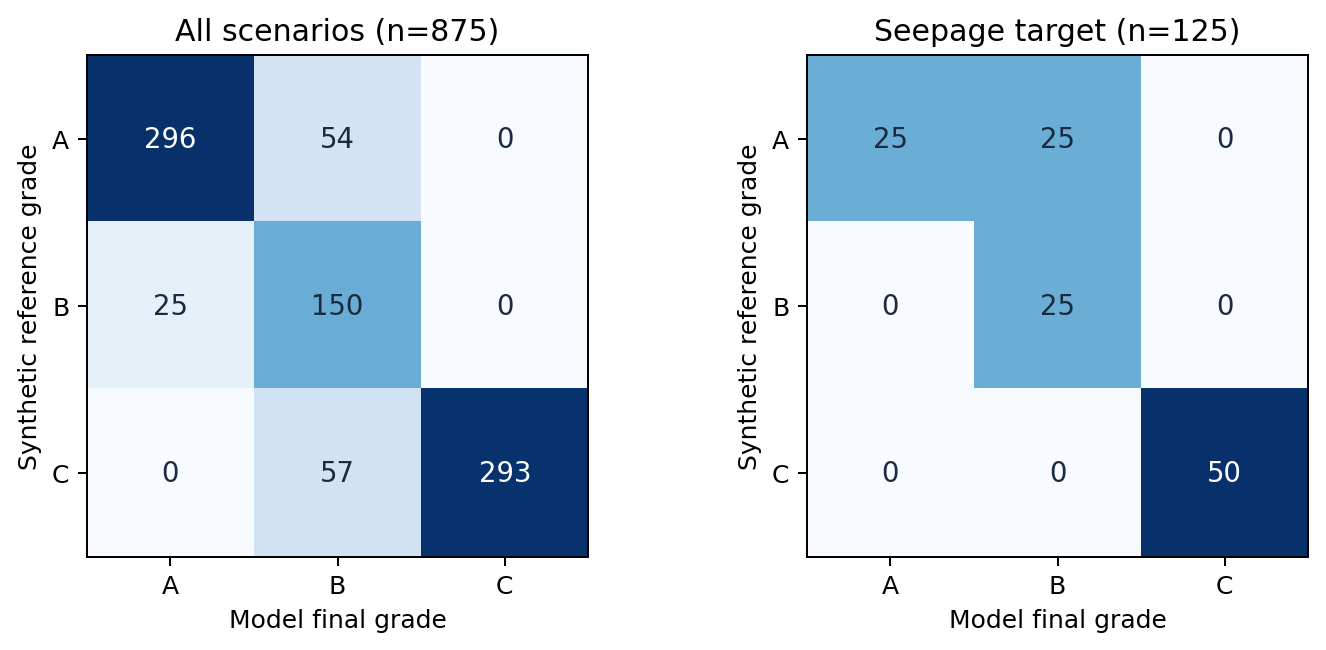
\includegraphics[width=\columnwidth]{overall_confusion.png}
\caption{Overall and seepage-target confusion matrices in the controlled benchmark.}
\label{fig:confusion}
\end{figure}

\subsection{Machine-learning comparison}
Table~\ref{tab:ml} compares the rule chain and grouped five-fold OOF machine-learning models. The shallow tree underperformed the rule baseline on all aggregate metrics. Majority-vote random forest increased C recall from 0.8371 to 0.8543 and reduced C underestimates from 57 to 51, but its accuracy and macro-F1 were lower than those of the rule chain. Thus, the machine-learning layer is useful as a nonlinear comparator and probability estimator, but not as a direct replacement for the physical rule chain. The physical-veto hybrid retained the safety direction of the rule chain while correcting a subset of its A/B errors: it reached 0.9257 accuracy, 0.9119 macro-F1, 0.9276 balanced accuracy, and 1.0000 C recall, with zero C underestimates and a safety loss of zero. It changed 154 of the 875 decisions relative to the RF threshold policy. The uncertainty-review fallback routed 62 records (7.09\%) to the rule-based fallback and achieved 0.9109 accuracy, 0.8964 macro-F1, 0.9657 C recall, and 12 C-to-B underestimates, with no direct C-to-A errors.

The hybrid's gain came from the decision layer rather than from an additional training signal. Relative to the RF threshold output, the physical lower bound changed 154 of 875 decisions, and the changes were constrained to prevent a downward movement in the ordinal risk scale. This makes the source of improvement auditable: the learned model supplies nonlinear ranking and upward corrections, while the existing rule chain supplies the admissibility floor. The result also explains why the hybrid should not be described as a pure machine-learning predictor; it is a constrained composition of a learned comparator and a physics-based safety rule.

\begin{table}[t]
\caption{Grouped five-fold OOF comparison on the 875 controlled records.}
\label{tab:ml}
\centering
\scriptsize
\begin{tabular}{lrrrrrr}
\toprule
Method & Acc. & mF1 & Bal. & Rec. C & C low & A high \\
\midrule
Rule baseline & .8446 & .8272 & .8467 & .8371 & 57 & 54 \\
Decision tree & .7074 & .6456 & .6352 & .6314 & 129 & 0 \\
RF majority & .8286 & .7835 & .7629 & .8543 & 51 & 0 \\
RF threshold & .8731 & .8584 & .8362 & .8571 & 50 & 0 \\
RF safety weight 6 & .7074 & .7009 & .6829 & 1.0000 & 0 & 179 \\
RF + physical veto & .9257 & .9119 & .9276 & 1.0000 & 0 & 54 \\
RF + veto + review & .9109 & .8964 & .9143 & .9657 & 12 & 54 \\
\bottomrule
\end{tabular}
\end{table}

\begin{figure}[t]
\centering
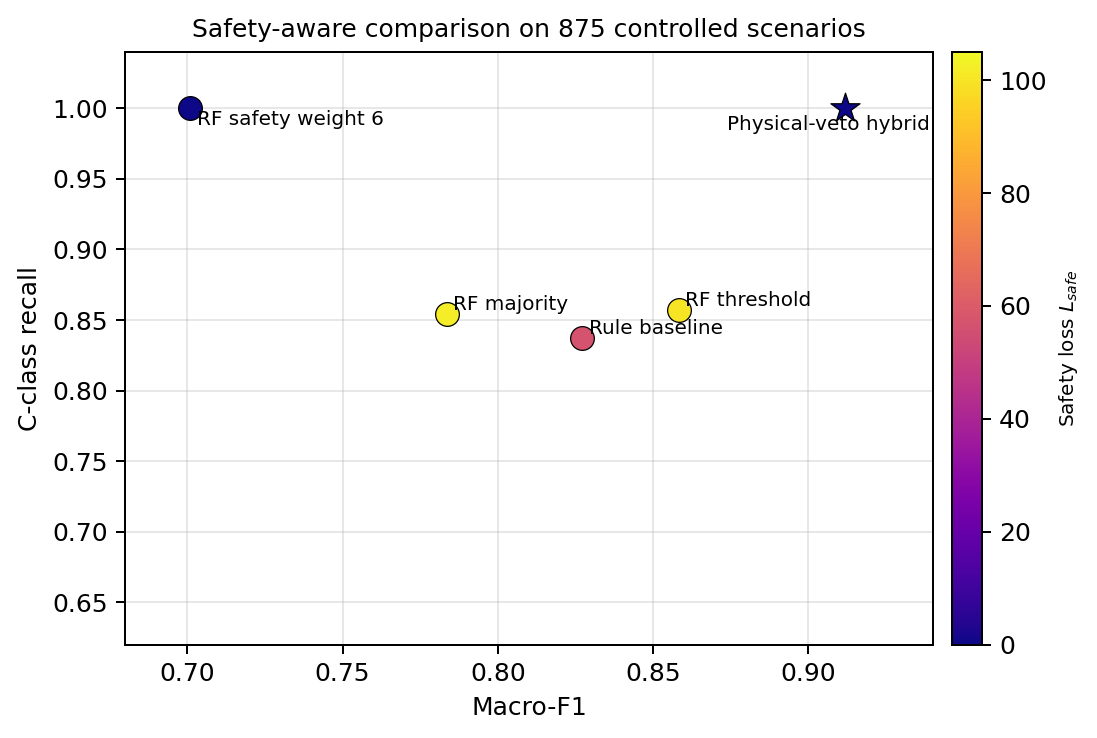
\includegraphics[width=\columnwidth]{ml_tradeoff.png}
\caption{Aggregate quality and critical-class recall for the rule and machine-learning policies. Color indicates the safety loss defined in Eq.~(\ref{eq:safeloss}).}
\label{fig:mltradeoff}
\end{figure}

\subsection{Pareto trade-off and nested validation}
A representative threshold $(\tau_C,\tau_B)=(0.35,0.20)$ reached 0.8731 accuracy, 0.8584 macro-F1, 0.8362 balanced accuracy, and 0.8571 C recall on the same OOF batch. Relative to the rule baseline, these are increases of 2.86, 3.12, and 2.00 percentage points for accuracy, macro-F1, and C recall, respectively. The improvement is not safety-neutral: all 50 C underestimates were direct C-to-A errors, producing $L_{\mathrm{safe}}=100$.

The finer $0.01$ threshold audit evaluated 10,000 pure RF policies. No threshold pair produced zero direct C-to-A errors. The best pure-RF macro-F1 point was $(0.19,0.06)$ with 0.8869 accuracy and 0.8900 macro-F1, but it still produced 50 direct C-to-A errors and $L_{\mathrm{safe}}=100$. This ablation makes the role of the physical lower bound explicit: the zero-C-to-A result is a property of the hybrid decision layer, not of RF thresholding alone.

A safety-priority class-weighted forest with C weight 6 achieved C recall 1.000 and zero C underestimates, but accuracy fell to 0.7074 and A overestimates rose to 179. This policy is not an engineering optimum; it represents one point on the risk--review-cost frontier. The threshold frontier is shown in Fig.~\ref{fig:pareto}.

\begin{figure}[t]
\centering
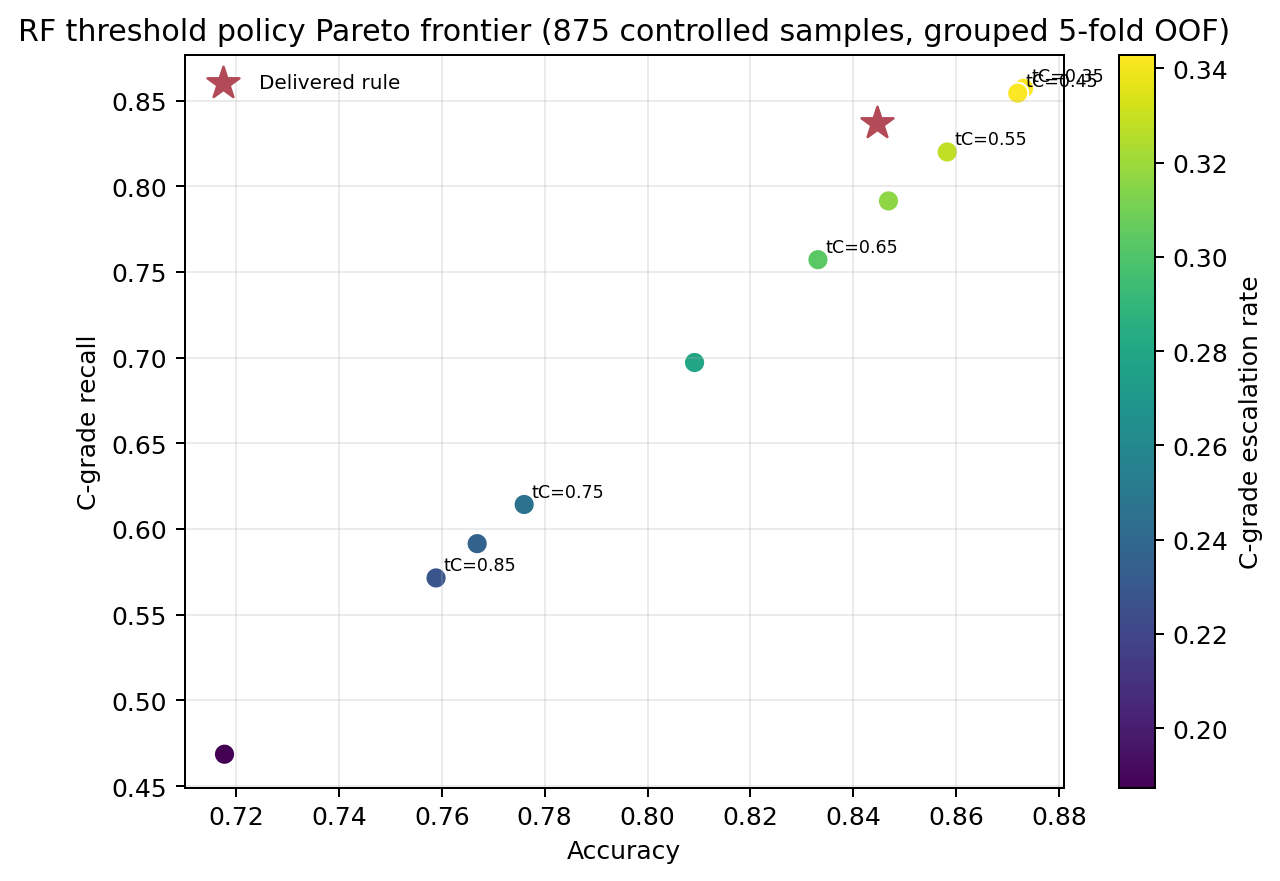
\includegraphics[width=\columnwidth]{pareto_frontier.png}
\caption{Threshold-policy Pareto frontier from grouped OOF random-forest probabilities. Color indicates escalation rate.}
\label{fig:pareto}
\end{figure}

A five-outer by three-inner grouped nested-validation prototype produced 0.8811 accuracy, 0.8704 macro-F1, 0.8495 balanced accuracy, and 0.8571 C recall, with 50 C underestimates in the pooled outer predictions. The persistence of direct C-to-A errors shows that selecting a C-recall constraint alone is insufficient. The physical-veto hybrid demonstrates one auditable implementation of a direct C-to-A hard constraint, while the review fallback quantifies the associated manual-review burden. Because both policies are evaluated on the same controlled generator, they should be treated as architecture evidence rather than as independent field performance.

The five-seed results provide a second check on direction rather than an external validation set. The hybrid's mean improvement over the paired rule baseline was 7.41 percentage points in accuracy and 7.65 percentage points in macro-F1, while the mean number of C underestimates decreased by 54.8. The consistency of these differences across generator realizations supports reproducibility of the decision-layer behavior. It does not remove the shared-generator limitation, because all five batches inherit the same feature construction, severity mapping, and rule logic.

\subsection{Multi-seed robustness}
To test sensitivity to the arbitrary generator realization, we regenerated five additional 875-record batches with seeds 20260930--20260934. The target construction, feature exclusion list, grouped five-fold split, forest hyperparameters, and threshold policy were unchanged; only the controlled-scenario random seed varied. These are independent generator realizations within the same synthetic family, not independent field labels. Table~\ref{tab:multiseed} reports mean$\pm$SD across the five batches. The delivered rule baseline remained stable at 0.8473$\pm$0.0017 accuracy and 0.8298$\pm$0.0017 macro-F1. The RF threshold policy reached 0.8754$\pm$0.0101 accuracy but retained 50.6$\pm$1.3 C underestimates and a safety loss of 101.2$\pm$2.7. The physical-veto hybrid reached 0.9214$\pm$0.0042 accuracy, 0.9064$\pm$0.0051 macro-F1, 0.9202$\pm$0.0062 balanced accuracy, and 0.9983$\pm$0.0038 C recall; C underestimates averaged 0.6$\pm$1.3. Paired with the rule baseline on the same five seeds, this corresponds to mean gains of 7.41, 7.65, and 7.12 percentage points in accuracy, macro-F1, and balanced accuracy, respectively, and a reduction of 54.8 C underestimates. The review fallback reduced C recall to 0.9691$\pm$0.0079 while routing 6.58$\pm$0.85\% of records to review. The small between-seed variation supports reproducibility of the decision-layer behavior within the generator family, but it does not establish transfer to field data.

\begin{table}[t]
\caption{Robustness across five additional generator seeds (mean$\pm$SD).}
\label{tab:multiseed}
\centering
\scriptsize
\resizebox{\columnwidth}{!}{%
\begin{tabular}{lcccccc}
\toprule
Method & Acc. & mF1 & Bal. & Rec. C & C low & $L_{\mathrm{safe}}$ \\
\midrule
Rule baseline & .8473$\pm$.0017 & .8298$\pm$.0017 & .8490$\pm$.0014 & .8417$\pm$.0016 & 55.4$\pm$.5 & 55.4$\pm$.5 \\
RF threshold & .8754$\pm$.0101 & .8621$\pm$.0150 & .8406$\pm$.0164 & .8554$\pm$.0038 & 50.6$\pm$1.3 & 101.2$\pm$2.7 \\
RF + physical veto & .9214$\pm$.0042 & .9064$\pm$.0051 & .9202$\pm$.0062 & .9983$\pm$.0038 & .6$\pm$1.3 & .6$\pm$1.3 \\
RF + veto + review & .9081$\pm$.0060 & .8924$\pm$.0071 & .9078$\pm$.0081 & .9691$\pm$.0079 & 10.8$\pm$2.8 & 10.8$\pm$2.8 \\
\bottomrule
\end{tabular}
}
\end{table}

\subsection{Review-budget sensitivity}
The manual-review threshold is itself an operational objective. We swept $u\in\{0.50,0.55,\ldots,0.90\}$, routing a hybrid prediction to the rule fallback when $\max_c p_c<u$. Across the five additional seeds, $u=0.50$ routed 1.53$\pm$0.67\% of records to review, achieved 0.9177$\pm$0.0057 accuracy, 0.9025$\pm$0.0066 macro-F1, 0.9903$\pm$0.0080 C recall, and a safety loss of 3.4$\pm$2.8 (range 0--6). It is feasible for the exploratory constraints of at most 5\% review and at most 6 safety-loss units in each seed batch. The earlier $u=0.60$ variant required 6.58$\pm$0.85\% review and yielded 0.9081$\pm$0.0060 accuracy, 0.8924$\pm$0.0071 macro-F1, and 10.8$\pm$2.8 safety-loss units. The original 875-record batch routed only 7 records at $u=0.50$ and retained the closed-set hybrid metrics. These thresholds are post-hoc operating points for protocol design; they must be fixed before an external evaluation.

\subsection{Inspection evidence as an evaluation state}
The nine field detections that entered manual review had confidence values between 0.4658 and 0.7770 and were all rejected as confirmed piping. The 13 artificial validation images produced 14 boxes with confidence values between 0.6699 and 0.9299, but the available package does not establish the positive boundary, missed detections, or a complete image-level truth table. Figure~\ref{fig:inspection} therefore reports the inspection evidence as a status distribution rather than as a field accuracy claim.

\begin{figure}[t]
\centering
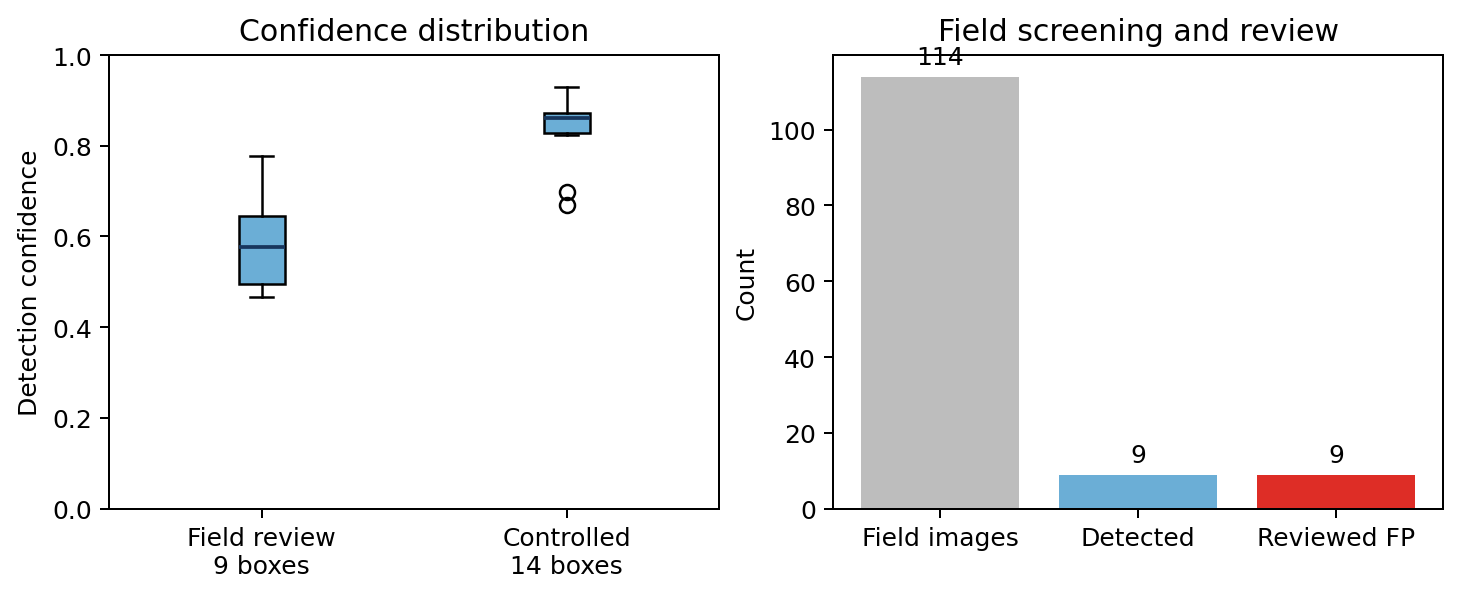
\includegraphics[width=\columnwidth]{inspection_review.png}
\caption{Inspection candidate confidence and manual-review status. The field review subset contains nine false positives; the artificial validation set contains 14 output boxes.}
\label{fig:inspection}
\end{figure}

The result has a direct implication for the C3 inspection indicator. An algorithmic candidate may trigger a review task, but it cannot be treated as a confirmed piping event until time, location, and manual status are closed. An unobserved image should remain unobserved rather than being encoded as no anomaly.

\section{Discussion}
The main methodological result is the explicit separation of physics, evidence state, and learned decision support. The reproduced rule baseline already performs well on the controlled benchmark, partly because hard gates are aligned with the generator's severity construction. A classifier trained on the same physical channels therefore faces a strong comparator. The random forest nevertheless provides a useful probability surface for exploring nonlinear interactions and operating points that cannot be expressed by a single score threshold.

This separation also clarifies the role of the digital twin. The three-dimensional geological scene and the simulated seepage field are not themselves a safety conclusion; they are context and evidence sources whose identity, spatial support, and validity interval must remain visible when an operational grade is produced. The proposed provenance graph provides a lightweight contract between the transparent-geology, transparent-computation, and transparent-inspection modules. It can therefore be implemented in a platform without making the visualization layer responsible for deciding whether an observation is confirmed, missing, or inapplicable.

The Pareto analysis changes the interpretation of ``improvement.'' The representative threshold policy improves accuracy and macro-F1 in the controlled batch, but it converts adjacent C-to-B errors into direct C-to-A errors. The physical-veto hybrid shows how this failure can be blocked without discarding the learned probability surface: the learned component remains responsible for upward corrections, while the rule chain supplies a safety floor. In levee safety, this is not a minor calibration detail. It is a change in the direction of error, and it should be represented as a separate objective or a hard admissibility condition. Conversely, the safety-priority policy prevents C underestimation by issuing many conservative A-to-B or A-to-C escalations. The correct operating point depends on the cost of review, the response capacity, and the consequence of a false-safe decision; a single scalar accuracy cannot determine it.

The field inspection records expose a second boundary. Candidate detection is not equivalent to defect confirmation. Water boundaries, vegetation, shadow, wet soil, and buildings can produce thermal patterns that resemble leakage or piping. The transparent evaluation interface therefore needs at least three states: candidate, reviewed status, and admissible evaluation input. This state model can support a digital twin without forcing incomplete evidence into a numerical grade.

The inspection finding is consistent with the remote-sensing literature's emphasis on registration and sensor context~\cite{Colomina2014}, and it has a direct design implication for future image models. A segmentation or detector can be optimized for candidate generation, but the evaluation layer should consume a reviewed event object with a location, time, confidence, and status. This allows the platform to retain useful false positives for retraining or inspection planning while preventing them from being promoted to confirmed piping in the current safety grade.

Several limitations remain. The 875 labels and the five additional seed batches are derived from the controlled severity design and are not independent field observations. The OOF threshold grid and the nested prototype remain exploratory, and the physical-veto hybrid uses the delivered rule output as a decision-layer safety floor. The engineering case has unresolved input conflicts, historical information leakage, and no independent physical re-run. The field images lack complete image-level truth and GPS-to-chainage linkage. The review-budget operating points were selected from the same controlled family and therefore should be regarded as protocol candidates rather than calibrated deployment thresholds. Consequently, the present study establishes reproducibility, failure modes, and a decision protocol, but not field-wide predictive accuracy, early-warning lead time, or a validated digital-twin closed loop.

\section{Conclusion}
We presented a safety-aware transparent evaluation framework for levee seepage stability that integrates geological evidence, seepage-field indicators, UAV inspection states, a physics-based rule chain, and a Pareto decision layer. The central result is a constrained composition rather than a replacement of physics by machine learning: the random forest supplies a nonlinear comparator, while the physical lower bound prevents a learned output from downgrading a rule-identified risk. On the original 875 controlled scenarios, this hybrid reached 0.9257 accuracy, 0.9119 macro-F1, and 1.0000 C recall with zero C underestimates; across five additional generator seeds it retained 0.9214$\pm$0.0042 accuracy, 0.9064$\pm$0.0051 macro-F1, and 0.9983$\pm$0.0038 C recall. A lower-review candidate at $u=0.50$ routed 1.53$\pm$0.67\% of records to review and retained 0.9903$\pm$0.0080 C recall within the same controlled family. These findings support the reproducibility and safety direction of the decision protocol, while the absence of independent field labels prevents a claim of engineering-optimal deployment.

The field inspection subset further showed that nine algorithmic candidates were all false positives after manual review. The appropriate platform behavior is therefore to preserve candidate, review, applicability, and missingness states and to expose the triggering evidence alongside the grade. Future work should complete the physical re-run of the engineering case, link inspection coordinates to levee chainage and hydraulic scenarios, obtain image-level truth labels, and evaluate the safety-constrained policies on independent field labels under a direct C-to-A hard constraint or reject option.

\section*{Acknowledgment}
The authors acknowledge the project team for providing the controlled evaluation package, engineering-case materials, and UAV inspection records. The author list and funding information will be completed after internal review.

\enlargethispage{5\baselineskip}\begin{thebibliography}{00}\tiny
\bibitem{GemPy} C. de la Varga, A. Schaaf, and T. H. W. Wellmann, ``GemPy 1.0: open-source stochastic geological modeling and inversion,'' \emph{Geoscientific Model Development}, vol. 12, pp. 1--32, 2019.
\bibitem{Richards} L. A. Richards, ``Capillary conduction of liquids through porous mediums,'' \emph{Physics}, vol. 1, pp. 318--333, 1931.
\bibitem{Breiman} L. Breiman, ``Random forests,'' \emph{Machine Learning}, vol. 45, pp. 5--32, 2001.
\bibitem{Quinlan} J. R. Quinlan, ``Induction of decision trees,'' \emph{Machine Learning}, vol. 1, pp. 81--106, 1986.
\bibitem{Deb} K. Deb, A. Pratap, S. Agarwal, and T. Meyarivan, ``A fast and elitist multiobjective genetic algorithm: NSGA-II,'' \emph{IEEE Transactions on Evolutionary Computation}, vol. 6, no. 2, pp. 182--197, 2002.
\bibitem{Xu} B. Xu, Z. Liu, R. Pang, et al., ``Data-driven collaborative safety evaluation for seepage reliability of embankments considering spatial variability,'' \emph{Journal of Hydrology}, vol. 660, p. 133490, 2025.
\bibitem{Schweckendiek} T. Schweckendiek, A. Vrouwenvelder, and E. Calle, ``Updating piping reliability with field performance observations,'' \emph{Structural Safety}, vol. 47, pp. 13--23, 2014.
\bibitem{Roscoe} K. Roscoe and A. Hanea, ``Bayesian networks in levee system reliability,'' in \emph{Proc. 12th Int. Conf. on Applications of Statistics and Probability in Civil Engineering}, Vancouver, Canada, 2015, pp. 1--8.
\bibitem{Chen} X. Chen, Y. Xu, H. Guo, et al., ``Comprehensive evaluation of dam seepage safety combining deep learning with Dempster--Shafer evidence theory,'' \emph{Measurement}, vol. 226, p. 114172, 2024.
\bibitem{Hou} Y. Hou, J. Yu, W. Liu, et al., ``Research on the full life cycle safety of levee based on BIM+mechanism algorithm,'' \emph{Archives of Civil Engineering}, vol. 72, no. 2, pp. 247--263, 2026.
\bibitem{Wellmann2018} F. Wellmann and G. Caumon, ``3-D structural geological models: Concepts, methods, and uncertainties,'' \emph{Advances in Geophysics}, vol. 59, pp. 1--121, 2018.
\bibitem{Celia1990} M. A. Celia, E. T. Bouloutas, and R. L. Zarba, ``A general mass-conservative numerical solution for the unsaturated flow equation,'' \emph{Water Resources Research}, vol. 26, no. 7, pp. 1483--1496, 1990.
\bibitem{vanGenuchten1980} M. T. van Genuchten, ``A closed-form equation for predicting the hydraulic conductivity of unsaturated soils,'' \emph{Soil Science Society of America Journal}, vol. 44, no. 5, pp. 892--898, 1980.
\bibitem{Baecher2003} G. Baecher and J. Christian, \emph{Reliability and Statistics in Geotechnical Engineering}. Chichester, U.K.: Wiley, 2003.
\bibitem{Colomina2014} I. Colomina and P. Molina, ``Unmanned aerial systems for photogrammetry and remote sensing: A review,'' \emph{ISPRS Journal of Photogrammetry and Remote Sensing}, vol. 92, pp. 79--97, 2014.
\bibitem{Ronneberger2015} O. Ronneberger, P. Fischer, and T. Brox, ``U-Net: Convolutional networks for biomedical image segmentation,'' in \emph{Proc. Medical Image Computing and Computer-Assisted Intervention}, 2015, pp. 234--241.
\bibitem{Redmon2016} J. Redmon, S. Divvala, R. Girshick, and A. Farhadi, ``You only look once: Unified, real-time object detection,'' in \emph{Proc. IEEE Conference on Computer Vision and Pattern Recognition}, 2016, pp. 779--788.
\bibitem{Hastie2009} T. Hastie, R. Tibshirani, and J. Friedman, \emph{The Elements of Statistical Learning}, 2nd ed. New York, NY, USA: Springer, 2009.
\bibitem{Saito2015} T. Saito and M. Rehmsmeier, ``The precision-recall plot is more informative than the ROC plot when evaluating binary classifiers on imbalanced datasets,'' \emph{PLoS ONE}, vol. 10, no. 3, p. e0118432, 2015.
\bibitem{Shafer1976} G. Shafer, \emph{A Mathematical Theory of Evidence}. Princeton, NJ, USA: Princeton University Press, 1976.
\bibitem{Fuller2020} A. Fuller, Z. Fan, C. Day, and C. Barlow, ``Digital twin: Enabling technologies, challenges and open research,'' \emph{IEEE Access}, vol. 8, pp. 108952--108971, 2020.
\bibitem{LundbergLee} S. M. Lundberg and S.-I. Lee, ``A unified approach to interpreting model predictions,'' in \emph{Advances in Neural Information Processing Systems}, vol. 30, 2017, pp. 4765--4774.
\end{thebibliography}
\end{document}








